% Macros pour la syntaxe


\chapter{Structured programming in {\alfa}}
\label{chapssubsystems}

\index{genericity}\index{structured programming}\index{program structures}\index{structures of programs}

\section{Introduction}

This chapter presents  generic and structured
programming in {\alfa}.

It first introduces the notion of \emph{size parameters} of an {\alfa}
system: a size parameter is a special index, often noted in capital
letters, used to give generic values to the size of the
problem. For example, when talking of a NxN matrix product, ``N'' is a
size parameter. In an {\alfa} system, such a parameter will appear in
the domains and affine functions as an index which is global to all
the domains of the system. The reader may already have noticed such
size parameters in some of the previous examples, as their use is
quite intuitive. This chapter will present them in greater detail.

The \emph{program structures} in {\alfa} are then introduced: so far
all the algorithms were simple enough to be described as a single
{\alfa} system, but one may want to structure a complex problem into
several smaller and simpler {\alfa} systems. The structure mechanisms
presented here allow this.
 

\section{Parameters\label{parameters}}

In most applications, it is useful to deal with \emph{parameterized}
algorithms. The polyhedral SARE model allows for a simple but powerful
parameter scheme which is demonstrated in the following program, a
simple matrix-vector product.

\begin{verbatim}
system matvect :{N | N>1}                               -- 1  
               (M : {i,j | 1<=i,j<=N} of real;          -- 2  
                V : {j | 1<=j<=N} of real)              -- 3  
       returns (R : {i | 1<=i<=N} of real);             -- 4  
var                                                     -- 5  
  C : {i,j | 1<=i,j<=N} of real;                        -- 6  
let                                                     -- 7  
  C = case                                              -- 8  
        {i,j | j=0} : 0.(i,j->);                        -- 9  
        {i,j | j>0} : C.(i,j->i,j-1) + M * V.(i,j->j);  -- 10 
      esac;                                             -- 11 
  R = C.(i->i,N);                                       -- 12 
tel;                                                    -- 13 
\end{verbatim}

In this system, \texttt{N} is a \emph{size parameter}\index{size
parameters}\index{parameters} which is declared in the header of the
system using  a \emph{parameter domain},\index{parameter
domain}\index{domain of the parameters} here \texttt{\{N |N>1\}}. This
parameter domain may be any {\alfa} domain, in particular there is no
limit on the number of parameters, and this domain may express any
affine inequation between the parameters. For example, \texttt{\{M,N|
M<2N\}} is a valid parameter domain.

Such a parameter may then appear anywhere in the system where indices
are allowed, that is, in domains (see lines~2-4 of
the previous program) and in affine functions (see line~12).

This parameterization retains all the properties of the language, for
parameters are actually special indices which are shared by all the
variables and subexpressions of a system. For example the
parameterized domain of the variable \texttt{M}, defined line~2 as
\texttt{\{i,j| 1<=i,j<=N\}}, actually denotes the domain
\texttt{\{i,j,N| 1<=i,j<=N\}}. Similarly, the parameterized affine
function \texttt{(i->i,N)} of line~12 actually represents the closed
function \texttt{(i,N->i,N,N)}. Thus a parameterized system is nothing
but a usual SARE where all the objects share the parameter
indices. Actually the system manipulated by {\mmalfa} is the
following:

\begin{verbatim}
system matvect                                                    -- 1  
               (M : {i,j,N | 1<=i,j<=N} of real;                  -- 2  
                V : {j,N | 1<=j<=N} of real)                      -- 3  
       returns (R : {i,N | 1<=i<=N} of real);                     -- 4  
var                                                               -- 5  
  C : {i,j,N | 1<=i,j<=N} of real;                                -- 6  
let                                                               -- 7  
  C = case                                                        -- 8  
        {i,j,N | j=0} : 0.(i,j,N->);                              -- 9  
        {i,j,N | j>0} : C.(i,j,N->i,j-1,N) + M * V.(i,j,N->j,N);  -- 10 
      esac;                                                       -- 11 
  R = C.(i,N->i,N,N);                                             -- 12 
tel;                                                              -- 13 
\end{verbatim}



\section{Structures\label{structures}}

\index{structured programming}\index{program structures}\index{structures of programs}
The issue of structuring a complex algorithm into a hierarchy of SAREs
is more complex than it seems. Obviously, it is partly addressed by
the decomposition of the problem into equations: it is always possible
to break an equation into two simpler equations, using an auxilliary
variable to hold a subexpression of the initial expression. The
reverse operation, replacing a variable appearing in an expression
with its definition, is also always possible. The {\mmalfa}
environment provides assistance for both these operations, thus ensuring
that the resulting system is equivalent to the initial one\footnote{These
operations are similar to $\beta$-conversion in the
lambda-calculus.}.\index{beta conversion}

Structuring using equations, however, basically remains first-order
structuring (in the usual functional meaning), and is thus
limited. These limits appear more clearly on the following example:
suppose we want to write in {\alfa} an algorithm for an
image processing application, which involves time-varying pixel matrices.
Such matrices are represented in {\alfa} as three-dimensional data
arrays (two matrix dimensions, and one -- possibly unbounded -- time
dimension) as represented on Fig.\ref{CollectionLineaire}.
\index{time-varying matrices}
\begin{figure}[!t]
  \centerline{
    \includegraphics{figures/matcoll}
  }
\caption{Linear collection of bidimensional matrices
\label{CollectionLineaire}}
\end{figure}

Now let us try to re-use the equations of the matrix-vector product to
operate on these time-varying matrices. Obviously it is not possible
in a straightforward manner, for the inputs don't have the proper
dimension. For example we will need to rewrite the whole of the
equation defining \texttt{C} to add one dimension to the domains and
the affine functions, yielding the following equation:

\begin{verbatim}
  C = case                                                       -- 8  
        {i,j,t | j=0}: 0.(i,j,t->);                              -- 9  
        {i,j,t | j>0}: C.(i,j,t->i,j-1,t) + M * V.(i,j,t->j,t);  -- 10 
      esac;                                                      -- 11 
\end{verbatim}

Structuring with variable will never be adequate when such a
\emph{dimension extension} \index{dimension extension}is needed, which
is the usual case.  The remainder of this chapter presents the {\alfa}
program structures addressing this problem.



\section{Simple structures} 

Let us try and write an {\alfa} SARE for the addition of two integers
(or fixed-point numbers) written in binary notation.  Such a binary
addition is classically described as a sequence of \emph{full adder}
operations with the propagation of a carry bit from one full adder to
the following, as described by Fig.\ref{adder}.
\index{adder}\index{binary addition}

\begin{figure}[!ht]
  \centerline{
    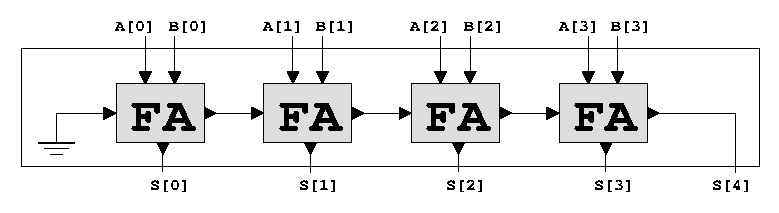
\includegraphics{figures/adder}
  }
\caption{Addition of integers coded in boolean, using \emph{full adders}\label{adder}}
\end{figure}

The following system is a \emph{full adder} function written in {\alfa}. 
\index{full adder}

\begin{verbatim}
      system FullAdder (A,B,Cin : boolean) 
               returns (X,Cout : boolean);
      let
        X = A xor B xor Cin;
        Cout = (A and B) or (A and Cin) or (B and Cin);
      tel;
\end{verbatim}



To build an adder system with this program, we need to be able to
express that we have a linear collection of instances of this system,
as shown in Fig.\ref{adder}. The shape of this linear collection may
be expressed as an {\alfa} domain, say \texttt{\{b|0<=b<W\}} where
\texttt{W} is a size parameter giving the number of bits.
\index{use statement}

The structure construct \textbf{use} in {\alfa} allows precisely that:
the following system describes in {\alfa} the adder given Fig.\ref{adder}: 
\index{adder}\index{binary addition}

\begin{verbatim}
     system Plus: {W|W>1} (A,B: {b| 0<=b<W} of boolean)         -- 1  
                  returns (S : {b| 0<=b<=W} of boolean);        -- 2  
     var                                                        -- 3  
       Cin, Cout, X : {b| 0<=b<W} of boolean;                   -- 4  
     let                                                        -- 5  
       use {b| 0<=b<W} FullAdder[] (A,B,Cin) returns(X, Cout);  -- 6  
       Cin[b] =                                                 -- 7  
         case                                                   -- 8  
           {| b=0} : 0[];                                       -- 9  
           {| b>0} : Cout[b-1];                                 -- 10 
         esac;                                                  -- 11 
       S[b] =                                                   -- 12 
         case                                                   -- 13 
           {| b<W} : X;                                         -- 14 
           {| b=W} : Cout[W-1];                                 -- 15 
         esac;                                                  -- 16 
     tel;                                                       -- 17 
\end{verbatim}


\index{use statement}
In this system, the line 6 reads as follows: ``Use a collection of
instances of the subsystem \texttt{FullAdder}. This collection has the
shape of the extension domain\index{extension domain} \verb!{b|0<=b<W}! 
and is thus indexed by index \texttt{b}. Let the inputs of
the \texttt{b}-th instance be the variables \texttt{A}, \texttt{B} and
\texttt{Cin} at point
\texttt{b}, and similarly let the outputs of this collection of
instances be the variables \texttt{X} and \texttt{Cout}.''
(The lines~7-11 describe the carry propagation, and lines~12-16
define the output of this binary adder.)

\index{dimension extension}
In other words, line~11 is a shortcut for the following equations,
which are those of the system \texttt{FullAdder} whith the dimension
of the variables extended from zero to one:

\begin{verbatim}
        X[b] = A[b] xor B[b] xor Cin[b];
        Cout[b] = (A[b] and B[b]) or (A[b] and Cin[b]) or (B[b] and Cin[b]);
\end{verbatim}





\section{Syntax of the \emph{use} construct}

\index{use syntax}
The \textbf{use}\ construct appears at the syntactic
level of an equation, since it is basically a shortcut for a set of
equations. Here is the general syntax of an equation/use:
{\tt
\begin{tabbing}
xxx\= xxx\= xxx\= xxx\= xxx\= xxx\= xxx\= xxx\= xxx\=  \kill
\textsl{Equation} ::\\
\>\> \textsl{Identifier} = \textsl{Expression} ;\\
\> \Alt\ \> use \Opt{ \textsl{ExtensionDomain}} \textsl{Identifier}\\
\>\>\>\>\>\> \Opt{[\textsl{ParamAssignment} ]} \\
\>\>\>\>\>\>( \textsl{ExpressionList} )\\
\>\>\> returns\>\>\> ( \textsl{IdentifierList} ) ;
\end{tabbing}
}
 

\index{parameter assignment}\index{assignment of the
parameters}\index{parameters}
In this syntax we see that there is an optional \emph{parameter
assignment} which is discussed in the following.
In the previous addition, the subsystem \texttt{FullAdder} has
no parameters, and the parameter assignment is therefore empty. 




\section{Binary multiplication in {\alfa}}

When performed by hand, a multiplication is basically a collection
of additions, as shown by Fig.\ref{intmul}. \index{binary multiplication}

\begin{figure}[!ht]
\begin{center}
    \includegraphics{figures/intmul}
  \caption{Product of two fixed point reals in binary representation\label{intmul} }
\end{center}
\end{figure}


The following program is the {\alfa}
incarnation of Fig.\ref{intmul}. Line~8 performs the binary product of
all the bits of the first operand by each bit of the second. Line~10
describes a linear collection of additions, indexed by \texttt{m}
which is the row index in Fig.\ref{intmul}. Lines~12-17 link the
result of one additions to the input of the following. 

\begin{verbatim}
    system Times: {W|W>2} (A,B: {b| 0<=b<W} of boolean)   -- 1  
                  returns (X  : {b| 0<=b<W} of boolean);  -- 2  
    var                                                   -- 3  
      P : {b,m| 0<=b,m<W } of boolean;                    -- 4  
      Si : {b,m| 0<=b<W; 0<m<W } of boolean;              -- 5  
      So : {b,m| 0<=b<=W; 0<m<W } of boolean;             -- 6  
    let                                                   -- 7  
      P[b,m] = A[b] and B[m];                             -- 8  
      use {m| 0<m<W} Plus[W] (Si,P) returns (So);         -- 9   
                                                          -- 10 
      Si[b,m] =                                           -- 12 
                                                          -- 11
        case                                              -- 13 
          {| m=1} : P[b,m-1];                             -- 14 
          {| m>1} : So[b+1,m-1];                          -- 15 
        esac;                                             -- 16 
      X[b] = So[b+1,W-1];                                 -- 17 
    tel;                                                  -- 18 
\end{verbatim}


Here the parameter assignment \texttt{W} just equates the bit size
parameter of the subsystem \texttt{Plus} and that of the
multiplication. In the general case, however, this parameter
assignment may be any affine function, which proves very
powerful. Figure~\ref{accumdraw} describes the problem of accumulating
binary numbers without overflow: the sum of two $N$-bits numbers may
be a $N+1$ bits number, therefore we need to use additions of
increasing sizes to avoid loss of bits. This is expressed in {\alfa} as:
\begin{verbatim}
         use {i| 1<=i<N} Plus[W+i-1] (A1,A2) returns (Acc);
\end{verbatim}
\index{parameter assignment}\index{assignment of the
parameters}\index{parameters}
\begin{figure}[!ht]
\centerline{
   \includegraphics{figures/Accum}
    }
\caption{Binary numbers accumulation. \label{accumdraw} }
\end{figure}

Another example where the natural structuring of an algorithm
makes use of a parameter assignment depending on the extension indices
is the Gaussian elimination given at the beginning of
chapter~\ref{static}. The reader is invited to try and understand this
program.

\index{extension domain}
Note that in all our examples, the extension domain is
monodimensional, but this is not a rule: in the general case the
extension domain may be any arbitrary {\alfa} domain. For example, in
an image processing application, a 2-dimensional extension domain may
be used to apply some function to all the points of an image.

\section{Manipulating structured programs}

A structured program is stored in {\mmalfa} as a {\mma} list of
systems called a \emph{library}. The default library is stored in the
global variable \verb!$library!.\index{$library}

A structured program may be written in one single file or several
distinct files.  In the latter case the \texttt{load[]} function
returns a library composed of all the systems contained in the file,
and stores this library in \verb!$library!. %$ 

If the program is stored in several files, it is the responsibility of
the user to build a proper library, i.e. a {\mma} list of all the
systems needed by the hierarchical structure of the program. For this
purpose, the user will typically use {\mma} list manipulating
functions such as \texttt{Join[], Append[]}...\index{structured
programs}

In addition, two functions, \texttt{putSystem[]} and
\texttt{getSystem[]}, may be used to extract a system from a library
and to put back a modified system in a library. Typically one of the
system is extracted from the library, modified by some program
transformation, and then put back in the library.\index{putSystem[]}\index{\getSystem[]}




\section{Program transformations associated with structures}

Most {\mmalfa} functions handle parameterized programs and \emph{use}
statements. There are, however, some major exceptions such as the
\texttt{writeC[]} translator. \index{writeC[]}In this case, {\mmalfa}
provides program transformations transforming a structured program
into a simpler equivalent one~:

\begin{itemize}

\item \texttt{assignParameterValue[]} \index{assignParameterValue[]}
gives a value to a size parameter, i.e. it refines a generic system
into a specialized one.

\item \texttt{inlineSubSystem[]} \index{inlineSubSystem[]} expands a
\emph{use} statement, replacing it with the equations of the
corresponding subsystem, properly modified to take the dimension
extension into account.\index{flattenning a structured program}

\item \texttt{inlineAll[]} \index{inlineAll[]} recursively flattens a
structured {\alfa} program.

\end{itemize}











